\documentclass{beamer}

\usepackage{tikz}
\usepackage{graphicx}
\usepackage{caption}

\begin{document}
\captionsetup{font=scriptsize, labelfont=scriptsize}
\setbeamertemplate{caption}{\raggedright\insertcaption\par}

\title{Frequent-Collision Blockchains for Local Geographic Authentication}
\author{Ryan Robinett and Tiago Royer}
\date{10 Dec 2019}
\institute[CMSC33300]{
    CMSC33300 --- Networks \\
    Department of Computer Science \\
    University of Chicago
}

\begin{frame}
    \titlepage
\end{frame}

\begin{frame}
	\frametitle{Problem motivation}

	\begin{itemize}
		\item Geographic Authentication:
			proving you are/were in a certain location
			at a certain point in time
		\item Goal: decentralized, historic geographic authentication
			\begin{itemize}
				\item Conventional geographic authentication asks, \textbf{``Where are you now?''}
				\item We want to ask, \textbf{``Where have you been in the recent past?''}
			\end{itemize}
		\item Proposed Solution:
			\begin{itemize}
				\item Peer-to-peer ``checkins'' over a \textbf{smartphone
					\textit{ad hoc} network (SPAN)}
				\item Store checkins using a \textbf{blockchain}
				\item Due to disconnectedness of SPANs, this blockchain will
					inevitably \textbf{fork}; want to use this as a feature,
					rather than a bug
			\end{itemize}
	\end{itemize}
\end{frame}

\begin{frame}
	\frametitle{Blockchains and Forking}

	\begin{columns}{}
		\begin{column}{0.5\textwidth}
			\begin{figure}
				\centering
				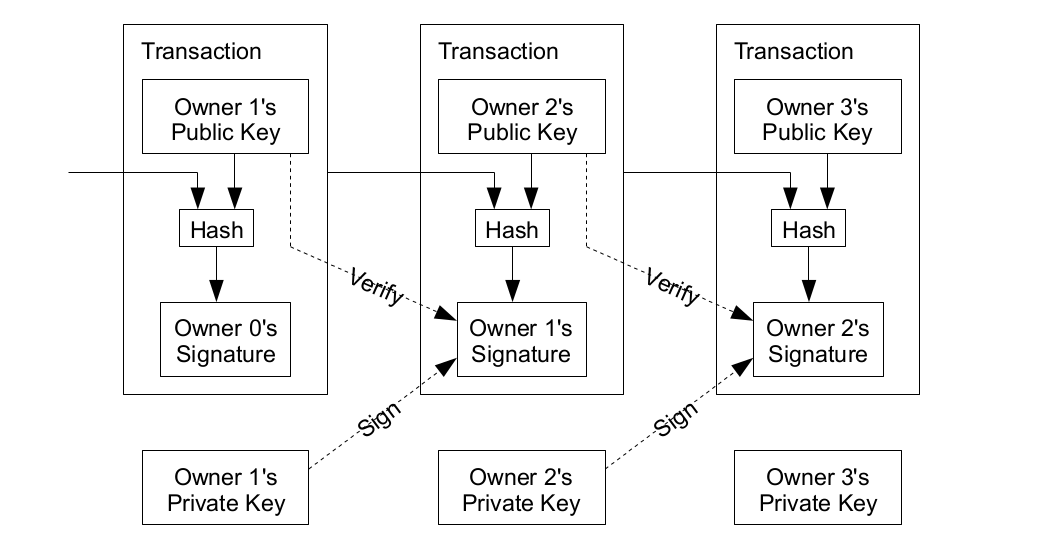
\includegraphics[width=\textwidth]{nakamoto_hashes.png}
				\caption{Nakamoto 2008}
			\end{figure}

			\begin{figure}
				\centering
				\vspace{-1cm}
				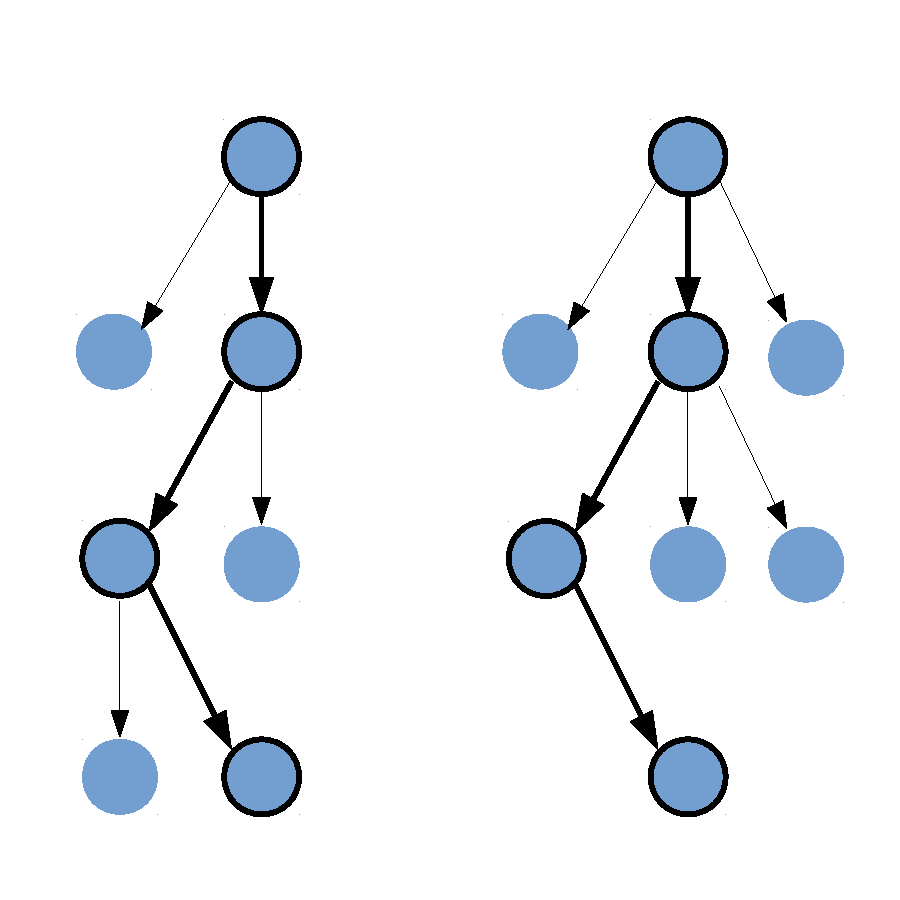
\includegraphics[width=0.5\textwidth]{fork_fig.pdf}
				\caption{Though local copies of the blockchain differ,
					they ``eventually'' agree identically on the
					\textbf{global chain}}
			\end{figure}
		\end{column}

		\begin{column}{0.5\textwidth}
			\begin{itemize}
				\item The Bitcoin blockchain is the prototypical blockchain
				\item Distinct nodes in the Bitcoin network each hold their
					own copy of the \textit{entire} history of transactions
				\item Each block must reference a pre-existing block using a hash function
				\item Guarantees \textbf{proof of work}
				\item Bitcoin ensures (in probability) that local copies of the blockchain
					will eventually agree on which chain is valid
			\end{itemize}
		\end{column}
	\end{columns}
\end{frame}

\begin{frame}
	\frametitle{Three networks evolving simultaneously}

	\begin{columns}
		\begin{column}{0.3\textwidth}
			\centering
			\textbf{SPAN}
			\begin{figure}
				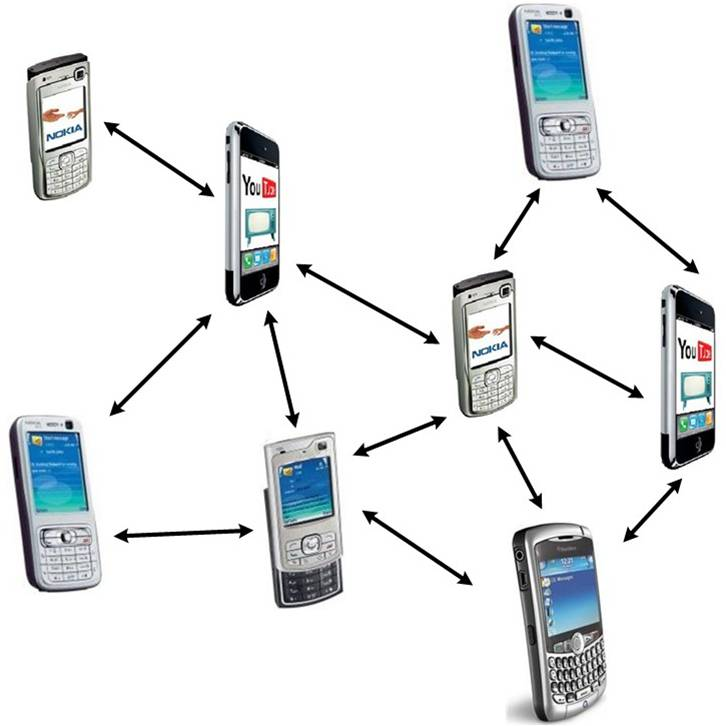
\includegraphics[width=\textwidth]{span.jpg}
			\end{figure}
			\begin{scriptsize}
				\begin{itemize}
					\item Nodes enter/leave the network all the time
					\item Network essentially always fragmented
				\end{itemize}
			\end{scriptsize}
		\end{column}

		\vrule{}

		\begin{column}{0.3\textwidth}
			\centering
			\textbf{Local Blockchain \\ (for each node)}
			\begin{figure}
				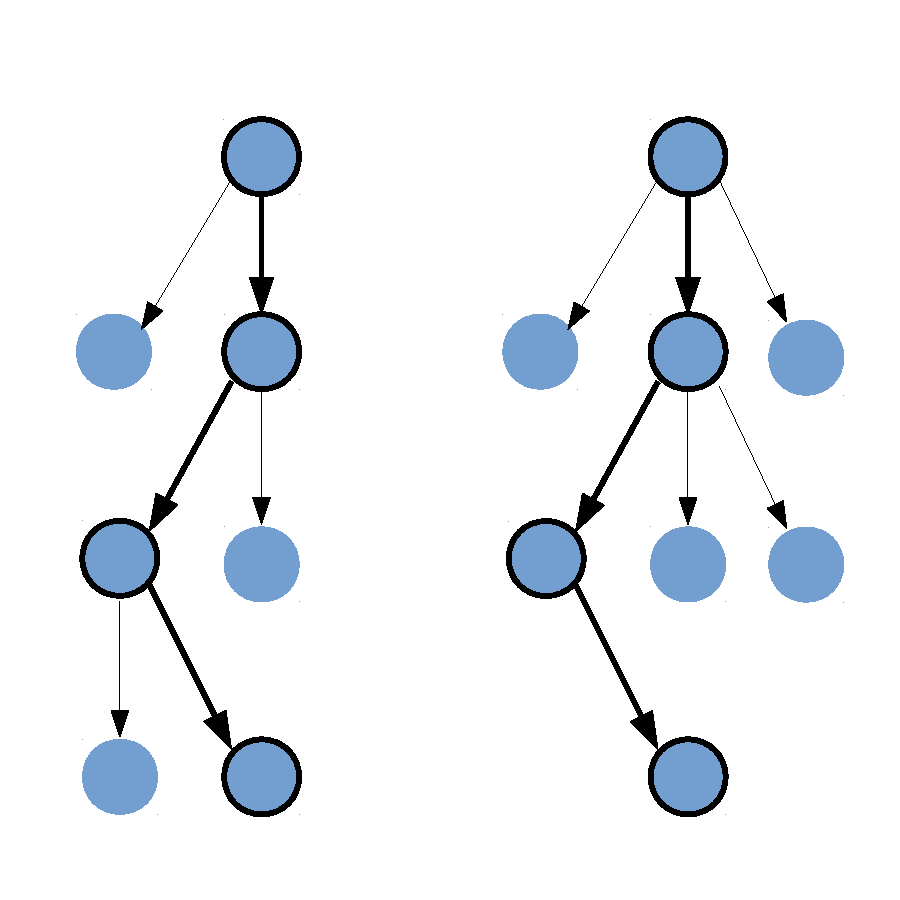
\includegraphics[width=\textwidth]{fork_fig.pdf}
			\end{figure}
			\begin{scriptsize}
				\begin{itemize}
					\item Unique tree of blocks for each node
					\item Tree growth contingent on the ``checkins'' to which
						node is privy
				\end{itemize}
			\end{scriptsize}
		\end{column}

		\vrule{}

		\begin{column}{0.4\textwidth}
			\centering
			\textbf{Global Blockchain...?}
			\begin{scriptsize}
				\begin{itemize}
					\item Conventionally, induced as the set-theoretic
						intersection of all local blockchains...
					\item But we are no longer guaranteed that this
						intersection would be a tree, or even if it would
						be well-defined
					\item Per Nakamoto: For each node,
						there exists a neighborhood of nodes for which
						a global chain (at least among these neighbors) is
						well-defined
					\item \textbf{Hope:} Each such \textbf{neighborhood chain}
						corresponds to interaction of nodes within
						geographic proximity over some appreciable timescale
				\end{itemize}
			\end{scriptsize}
		\end{column}
	\end{columns}
\end{frame}

\begin{frame}
	\frametitle{What we accomplished:}

	\begin{enumerate}
		\item \textbf{Write protocol that allows for the formation of
			blockchains in the manner described}
			\begin{itemize}
				\item Must be robust to first-order
					adversarial behavior
			\end{itemize}
		\item \textbf{Simultaneously simulate SPAN and local blockchains
			under this protocol}
			\begin{itemize}
				\item Simulate evolution of SPAN using \textbf{random
					geometric graphs}
				\item Run blockchain protocol as the SPAN evolves to
					create varying local chains
				\item Tune parameters so that protocol creates
				neighborhood chains corresponding to geographic
				locales
			\end{itemize}
	\end{enumerate}
\end{frame}

\begin{frame}
	\frametitle{1) The Protocol}
	\begin{columns}
		\begin{column}{0.3\textwidth}
			\hfil
			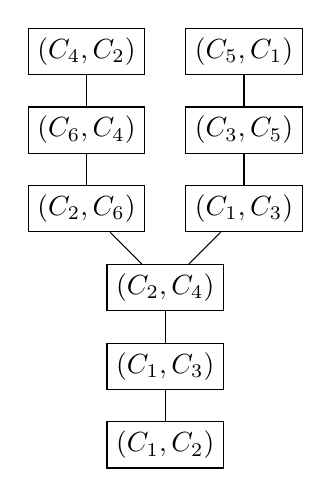
\begin{tikzpicture}[
					every node/.style = {
						shape = rectangle,
						draw,
						minimum width = 1cm,
						minimum height = 0.5cm,
					},
			]
				\draw (0, 0) node (a1) [rectangle] {$(C_1, C_2)$};
				\draw (0, 1) node (a2) [rectangle] {$(C_1, C_3)$};
				\draw (0, 2) node (a3) [rectangle] {$(C_2, C_4)$};
				\draw (1, 3) node (b4) [rectangle] {$(C_1, C_3)$};
				\draw (1, 4) node (b5) [rectangle] {$(C_3, C_5)$};
				\draw (1, 5) node (b6) [rectangle] {$(C_5, C_1)$};
				\draw (-1, 3) node (c4) [rectangle] {$(C_2, C_6)$};
				\draw (-1, 4) node (c5) [rectangle] {$(C_6, C_4)$};
				\draw (-1, 5) node (c6) [rectangle] {$(C_4, C_2)$};

				\draw (a1) -- (a2);
				\draw (a2) -- (a3);
				\draw (a3) -- (b4);
				\draw (b4) -- (b5);
				\draw (b5) -- (b6);
				\draw (a3) -- (c4);
				\draw (c4) -- (c5);
				\draw (c5) -- (c6);
			\end{tikzpicture}
		\end{column}

		\begin{column}{0.7\textwidth}
			\begin{itemize}
				\item Cryptographic challenge: Tuple $(t_C, k_C)$
					\begin{itemize}
						\item $k_C$ is the public key of the creator
						\item $t_C$ is timestamp of the problem creation
					\end{itemize}
				\item Block: Tuple $(t_C, t_S, k_S, n, b)$
					\begin{itemize}
						\item $(t_C, t_S)$ is a cryptographic challenge
						\item $k_S$ is the timestamp of the solution
						\item $k_S$ is the public key of the solver
						\item $n$ is the solution nonce
						\item $b$ is a pointer to a previous block
					\end{itemize}
				\item Hashing: $H(t_C t_S k_S n b) < \tau$
				\item Nodes exchange cryptographic challenges
				\item Handshakes are recorded in the ledger
					in the form of blocks
			\end{itemize}
		\end{column}
	\end{columns}

\end{frame}

\begin{frame}
	\frametitle{2) The Simulation}

	\begin{columns}
		\begin{column}{0.3\textwidth}
			\centering
			
		\end{column}

		\begin{column}{0.7\textwidth}
			\centering

		\end{column}
	\end{columns}	
\end{frame}

\begin{frame}
	\frametitle{2) The Simulation}

	
\end{frame}

\begin{frame}
	\frametitle{Supplementary Material: Transaction Primitives}
	\begin{figure}
		\scriptsize
		\centering
		\textbf{Transaction Primitives:} \\
		\vspace{5mm}
		\begin{description}
			\item[\textbf{Challenge Proposal:}] A challenge proposal $\mathcal{P}$ by
				node $C$ is a tuple of the form
				$$\mathcal{P}=(t_{\mathcal{P},C},\mathcal{C};\mathcal{P}^\prime_h,\mathcal{P}^\prime_t).$$
				Here:
				\begin{itemize}
					\item $t_{\mathcal{P},C}$ is the timestamp of $C$'s local clock upon
					creation of problem $\mathcal{P}$;
					\item $\mathcal{C}$ is the public key of node $C$;
					\item $\mathcal{P}^\prime_h$ is the header of block instance
					$\mathcal{P}^\prime$ (see below); and
					\item $\mathcal{P}^\prime_t$ is the tail of block instance
					$\mathcal{P}^\prime$. We refer to $\mathcal{P}^\prime$ as
					the \textbf{parent} of $\mathcal{P}$.
				\end{itemize}
				The tuple
				$\mathcal{P}=(t_{\mathcal{P},C},\mathcal{C};\mathcal{P}^\prime_h,\mathcal{P}^\prime_t)$
				naturally decomposes into the tuples
				$\mathcal{P}_h=(t_{\mathcal{P},C},\mathcal{C})$ and
				$\mathcal{P}_r=(\mathcal{P}^\prime_h,\mathcal{P}^\prime_t)$, which we
				refer to as the \textbf{header} and \textbf{reference tag} of $\mathcal{P}$,
				respectively.
			\item[\textbf{Block:}] A block $\mathcal{P}^*$ is a challenge proposal instance
				$\mathcal{P}=(t_{\mathcal{P},C},\mathcal{C};\mathcal{P}^\prime_h,\mathcal{P}^\prime_t)$
				together with the tuple $\mathcal{P}_t=(t_{\mathcal{P},S},\mathcal{S},n_{\mathcal{P},S})$.
				We refer to $\mathcal{P}^*_t$ as the \textbf{footer} of $\mathcal{P}^*$.
		\end{description}
	\end{figure}
\end{frame}

\end{document}
